% =======================================================================
\chapter{Metodología de trabajo}
\label{cap:metodologia}
% =======================================================================

Este capítulo describe cómo se construyó el trabajo: las decisiones de diseño
que delimitaron el estudio, el protocolo experimental y los criterios de
validación. El detalle formal de los algoritmos y el análisis de resultados
se encuentran en el paper del Capítulo~\ref{cap:paper}.

\section{Enfoque general}

El trabajo sigue un diseño factorial completo de dos factores:

\begin{itemize}
  \item \textbf{Factor A --- Problema} (5 niveles): Knapsack 0/1, TSP, CVRP,
    Flowshop y Job Shop.
  \item \textbf{Factor B --- Configuración de TS} (3 niveles): Básico,
    Intermedio y Avanzado.
\end{itemize}

El cruce produce quince módulos independientes. Sobre cada módulo se ejecutan
las instancias correspondientes y cinco semillas, para un total de
\textbf{360 experimentos} (Figura~\ref{fig:diseno_factorial}). La estructura
factorial permite atribuir diferencias al mecanismo y no al problema: al
mantener fija la instancia y variar solo el nivel, la diferencia de GAP mide
la contribución del mecanismo añadido.

\begin{figure}[H]
  \centering
  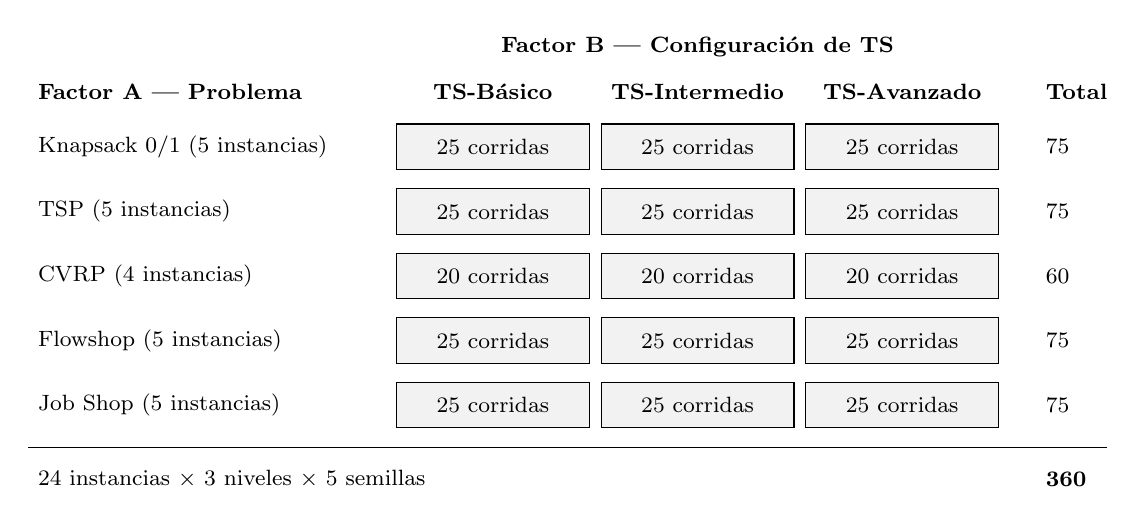
\begin{tikzpicture}[x=1cm, y=0.82cm,
      celda/.style={draw, minimum width=2.45cm, minimum height=0.58cm,
                    fill=gray!10, font=\footnotesize, inner sep=1pt},
      fila/.style={font=\footnotesize, anchor=west},
      tot/.style={font=\footnotesize, anchor=west}]
    % Encabezados
    \node[font=\footnotesize\bfseries] at (5.8,1.55)
      {Factor B --- Configuración de TS};
    \foreach \x/\n in {3.2/TS-Básico, 5.8/TS-Intermedio, 8.4/TS-Avanzado}
      \node[font=\footnotesize\bfseries] at (\x,0.85) {\n};
    \node[font=\footnotesize\bfseries, anchor=west] at (-2.7,0.85)
      {Factor A --- Problema};
    \node[font=\footnotesize\bfseries, anchor=west] at (10.1,0.85) {Total};
    % Filas: problema, instancias, corridas por celda, total por fila
    \foreach \y/\prob/\inst/\cel/\fil in {
        0/Knapsack 0\slash 1/5/25/75,
        -1/TSP/5/25/75,
        -2/CVRP/4/20/60,
        -3/Flowshop/5/25/75,
        -4/Job Shop/5/25/75}{
      \node[fila] at (-2.7,\y) {\prob\ (\inst\ instancias)};
      \foreach \x in {3.2, 5.8, 8.4}
        \node[celda] at (\x,\y) {\cel\ corridas};
      \node[tot] at (10.1,\y) {\fil};
    }
    % Total general
    \draw (-2.7,-4.65) -- (11.0,-4.65);
    \node[fila] at (-2.7,-5.15)
      {24 instancias $\times$ 3 niveles $\times$ 5 semillas};
    \node[tot, font=\footnotesize\bfseries] at (10.1,-5.15) {360};
  \end{tikzpicture}
  \caption{Diseño factorial del estudio. Cada celda es un módulo de Búsqueda
           Tabú (problema $\times$ nivel); sus corridas resultan de ejecutar
           cada instancia del problema con las cinco semillas.}
  \label{fig:diseno_factorial}
\end{figure}

\section{Decisiones de diseño}

Cuatro decisiones delimitan el estudio: comparar tres niveles acumulativos en
lugar de barrer parámetros, trabajar con cinco problemas de estructura
distinta, restringir el tamaño de las instancias y emplear únicamente
benchmarks públicos con mejor valor conocido. Las subsecciones siguientes
justifican cada una.

\subsection{Por qué tres niveles y no un barrido de parámetros}

Un barrido exhaustivo de hiperparámetros habría producido mejores GAP
absolutos, pero habría confundido el objetivo. Aquí interesa el efecto de
\emph{agregar un mecanismo}, no especificarlo en detalle. Por eso los tres
niveles son acumulativos —cada uno contiene al anterior más un componente
adicional— y los parámetros se fijan una única vez por problema, sin
re-ajuste por instancia.

\subsection{Por qué esos cinco problemas}

Los cinco problemas se seleccionaron por su heterogeneidad estructural. Cada
uno representa una familia distinta de POC —selección, ruteo y
secuenciación— y obliga a una codificación y a una vecindad propias
(Tabla~\ref{tab:problemas}). Los cinco son, además, problemas clásicos con
benchmarks públicos y mejor valor conocido documentado, requisito de la
métrica empleada. Un mecanismo que funciona en los cinco persigue una
generalidad que no tendría si se hubieran elegido cinco variantes de ruteo.

\subsection{Por qué instancias de tamaño moderado}

Se privilegiaron instancias de 50 a 150 elementos, que se obtienen de
benchmarks estándar. Instancias mayores habrían elevado el tiempo por
experimento por encima de la capacidad del hardware disponible (ver
Sección~\ref{sec:entorno}) y, con 360 corridas, el costo total se habría
vuelto prohibitivo. La contrapartida —que los resultados no informan sobre
escalabilidad— se reconoce explícitamente como limitación.

\subsection{Por qué benchmarks públicos con BKS conocido}

Usar instancias generadas \emph{ad hoc} habría impedido contrastar contra un valor
de referencia externo. Todas las instancias provienen de repositorios
públicos con mejor valor conocido (BKS) documentado~\cite{reinelt1991tsplib,
taillard1993benchmarks,christofides1979vehicle}. Esto permite expresar
el rendimiento como GAP y comparar entre problemas de unidades distintas.

\section{Instancias de prueba}

Se emplean 24 instancias. La Tabla~\ref{tab:instancias_tesis} resume su
procedencia; el detalle de tamaños y valores BKS está en el paper.

\begin{table}[H]
\centering
\caption{Origen de las instancias de prueba}
\label{tab:instancias_tesis}
\small
\begin{tabular}{llll}
\toprule
\textbf{Problema} & \textbf{Instancias} & \textbf{N.º} & \textbf{Fuente} \\
\midrule
Knapsack 0/1 & \texttt{knapPI\_11}--\texttt{knapPI\_15} & 5
             & Pisinger~\cite{pisinger2005hard} \\
TSP  & \texttt{eil51}, \texttt{berlin52}, \texttt{eil76},
       \texttt{kroA100}, \texttt{kroB100} & 5
     & TSPLIB~\cite{reinelt1991tsplib} \\
CVRP & \texttt{vrpnc1}--\texttt{vrpnc4} & 4
     & Christofides~\cite{christofides1979vehicle} \\
Flowshop & \texttt{ta001}, \texttt{ta011}, \texttt{ta021},
           \texttt{ta031}, \texttt{ta041} & 5
         & Taillard~\cite{taillard1993benchmarks} \\
Job Shop & \texttt{ft10} & 1
         & Fisher \& Thompson~\cite{fisher1963probabilistic} \\
         & \texttt{la01}, \texttt{la06}, \texttt{la11}, \texttt{la21} & 4
         & Lawrence~\cite{lawrence1984resource} \\
\midrule
\multicolumn{2}{l}{\textbf{Total}} & \textbf{24} & \\
\bottomrule
\end{tabular}
\end{table}

\section{Protocolo experimental}

El protocolo fija cuatro elementos antes de ejecutar los experimentos: la
solución inicial de cada problema, los parámetros de cada nivel, las semillas
junto con el criterio de parada, y la métrica de comparación. Fijarlos de
antemano asegura que los tres niveles se comparen en igualdad de condiciones.

\subsection{Soluciones iniciales}

Ningún nivel arranca desde una solución aleatoria. Cada problema emplea una
heurística constructiva determinista; así, la comparación entre niveles no
se distorsiona por la calidad del punto de partida:

\begin{table}[H]
\centering
\caption{Heurística constructiva por problema}
\label{tab:constructivas}
\small
\begin{tabular}{lp{9.2cm}}
\toprule
\textbf{Problema} & \textbf{Heurística inicial} \\
\midrule
Knapsack 0/1 & \emph{Greedy} por ratio ganancia/peso decreciente \\
TSP          & Vecino más cercano desde el nodo 0~\cite{johnson1997traveling} \\
CVRP         & Ahorros de Clarke-Wright~\cite{clarke1964scheduling} \\
Flowshop     & NEH (Nawaz, Enscore \& Ham)~\cite{nawaz1983heuristic} \\
Job Shop     & Decodificador Giffler-Thompson~\cite{giffler1960algorithms} con
               prioridad por tiempo total de procesamiento decreciente \\
\bottomrule
\end{tabular}
\end{table}

Esta decisión tiene una consecuencia visible en los resultados: en Flowshop,
donde NEH entrega una solución inicial de buena calidad, los tres niveles
de TS con vecindad de intercambio adyacente la mejoran poco.

\subsection{Parámetros por nivel}

Los parámetros se fijan por problema y nivel antes de ejecutar los
experimentos. La Tabla~\ref{tab:parametros_tesis} los resume; $|\mathcal{T}|$
es el tamaño de la lista tabú, $T_{\max}$ el número de iteraciones y $L$ el
umbral de estancamiento que dispara el reinicio.

\begin{table}[H]
\centering
\caption{Parámetros por problema y nivel}
\label{tab:parametros_tesis}
\small
\begin{tabular}{llccl}
\toprule
\textbf{Problema} & \textbf{Nivel} & $|\mathcal{T}|$ & $T_{\max}$ &
  \textbf{Reinicio} \\
\midrule
\multirow{3}{*}{Knapsack}
  & Básico  & 10 (fijo) & 500    & --- \\
  & Interm. & [5, 15]   & 1\,000 & $L=200$ \\
  & Avanz.  & [5, 15]   & 2\,000 & $L=200$, frecuencia \\
\midrule
\multirow{3}{*}{TSP}
  & Básico  & 10 (fijo) & 1\,000 & --- \\
  & Interm. & [5, 20]   & 2\,000 & $L=200$ \\
  & Avanz.  & [7, 25]   & 3\,000 & $L=300$, 4-opt \\
\midrule
\multirow{3}{*}{CVRP}
  & Básico  & 10 (fijo) & 1\,500 & --- \\
  & Interm. & [7, 20]   & 3\,000 & $L=300$ \\
  & Avanz.  & [7, 25]   & 5\,000 & $L=400$, frecuencia \\
\midrule
\multirow{3}{*}{Flowshop}
  & Básico  & 10 (fijo) & 2\,000 & --- \\
  & Interm. & [5, 20]   & 4\,000 & $L=500$ \\
  & Avanz.  & [5, 20]   & 5\,000 & $L=500$, frecuencia \\
\midrule
\multirow{3}{*}{Job Shop}
  & Básico  & 10 (fijo) & 2\,500 & --- \\
  & Interm. & [5, 15]   & 1\,000 & $L=200$ \\
  & Avanz.  & [5, 15]   & 1\,500 & $L=250$, frecuencia \\
\bottomrule
\end{tabular}
\end{table}

Nótese que en Job Shop el nivel Básico usa más iteraciones que los
posteriores. Es una decisión deliberada: el costo por iteración crece con la
lista dinámica, y mantener $T_{\max}$ constante habría hecho que los niveles
superiores consumieran un tiempo desproporcionado. El criterio fue igualar
aproximadamente el tiempo de cómputo, no el número de iteraciones.

\subsection{Semillas y criterio de parada}

Cada configuración se ejecuta con cinco semillas independientes,
$s \in \{42, 123, 456, 789, 1337\}$, y se reportan media y desviación
estándar. Aunque una corrida de TS es determinista una vez fijada la semilla,
esta gobierna los componentes estocásticos del algoritmo —desempates,
perturbaciones de reinicio y diversificación—. Cada semilla constituye así una corrida independiente.

Se eligen cinco semillas, y no un número mayor, como equilibrio entre el
costo computacional (360 experimentos) y la estimación de la variabilidad.
La baja desviación estándar observada (Figura~\ref{fig:dispersion}) respalda
esa elección.

El criterio de parada es el número máximo de iteraciones $T_{\max}$, sin
condición de convergencia adicional. Esto simplifica la comparación pero
implica que los tiempos no son directamente comparables entre problemas.

\subsection{Métrica de comparación}

Se emplea el GAP porcentual respecto al BKS definido en la
Ecuación~\ref{eq:gap_motivo}. Un GAP de \SI{0}{\percent} indica coincidencia exacta con el BKS. Un GAP negativo indicaría la \emph{superación} del BKS; no se observa en ninguno de los 360 experimentos. Las instancias de Flowshop se regeneran
desde las semillas publicadas por Taillard~\cite{taillard1993benchmarks}
(\texttt{instances/flowshop/generar\_taillard.py}) y sus BKS son
\emph{makespan} óptimos.

\section{Flujo de ejecución}

El experimento completo se ejecuta con un solo comando. El orquestador
recorre el producto cartesiano de problemas, instancias, algoritmos y
semillas, y persiste cada corrida en disco antes de agregar los resultados.
La Figura~\ref{fig:flujo_ejecucion} muestra ese flujo y el
Código~\ref{lst:orquestador}, su implementación.

\begin{figure}[H]
  \centering
  \begin{tikzpicture}[
      node distance=0.42cm,
      paso/.style={draw, rounded corners=2pt, align=center,
                   font=\footnotesize, text width=8.6cm,
                   minimum height=0.8cm, fill=gray!8},
      dec/.style={draw, diamond, aspect=3.4, align=center,
                  font=\footnotesize, inner sep=1pt, fill=gray!15},
      fl/.style={->, >=stealth, thick}]
    \node[paso] (cli)
      {\texttt{main.py -{}-all -{}-multi-seed}\\
       toma la siguiente combinación\\
       (semilla, problema, instancia, algoritmo)};
    \node[paso, below=of cli] (load)
      {\texttt{loader.py}: lee la instancia desde \texttt{instances/}\\
       y entrega la matriz de datos y el BKS};
    \node[paso, below=of load] (solve)
      {\texttt{runner.py}: importa el módulo de TS\\
       e invoca \texttt{solve(instance\_data, seed)}};
    \node[paso, below=of solve] (met)
      {\texttt{metrics.py}: calcula el GAP respecto al BKS};
    \node[paso, below=of met] (out)
      {Persiste la corrida en \texttt{output/}:\\
       \texttt{resultado.json} y \texttt{solucion.txt}};
    \node[dec, below=of out] (mas) {¿Quedan combinaciones?};
    \node[paso, below=of mas] (rep)
      {\texttt{reporter.py}: agrega las 360 corridas en \texttt{results/}\\
       (media y desviación estándar por instancia)};
    \node[paso, below=of rep] (fig)
      {\texttt{notebooks/} y \texttt{generar\_figuras.py}: tablas y figuras};
    \draw[fl] (cli) -- (load);
    \draw[fl] (load) -- (solve);
    \draw[fl] (solve) -- (met);
    \draw[fl] (met) -- (out);
    \draw[fl] (out) -- (mas);
    \draw[fl] (mas) -- node[right, font=\scriptsize]{no} (rep);
    \draw[fl] (rep) -- (fig);
    \draw[fl] (mas.east) -- ++(2.3,0)
      node[midway, above, font=\scriptsize]{sí} |- (cli.east);
  \end{tikzpicture}
  \caption{Flujo de ejecución del experimento completo. El ciclo superior se
           repite para las 360 combinaciones; la agregación y las figuras se
           generan una sola vez al final.}
  \label{fig:flujo_ejecucion}
\end{figure}

\lstinputlisting[caption={Orquestador de experimentos y opciones de línea de
comandos},label={lst:orquestador}]{codigos/05_orquestador.py}

El flujo de datos es lineal y sin estado compartido entre corridas:

\begin{enumerate}
  \item \texttt{loader.py} lee la instancia desde \texttt{instances/} y
    devuelve un diccionario con la matriz de datos y el BKS.
  \item \texttt{runner.py} invoca el \texttt{solve()} del módulo
    correspondiente con la semilla indicada.
  \item El resultado se persiste en
    \texttt{output/\{problema\}/\{instancia\}\_\{algoritmo\}\_\{fecha\}/}
    como \texttt{resultado.json} (valor, GAP, iteraciones, tiempo e historial
    de convergencia) y \texttt{solucion.txt}.
  \item \texttt{metrics.py} calcula el GAP y \texttt{reporter.py} agrega
    todas las corridas en \texttt{results/tabla\_consolidada.csv} con media y
    desviación estándar por instancia.
  \item Los cuadernos de \texttt{notebooks/} y el script
    \texttt{TESIS/generar\_figuras.py} producen las figuras a partir de esos
    CSV.
\end{enumerate}

Que cada corrida escriba su propio directorio con marca de tiempo permite
re-ejecutar experimentos sin sobrescribir resultados previos y auditar la
trazabilidad completa.

\section{Reproducibilidad}

La reproducción íntegra de los resultados requiere tres comandos:

\begin{verbatim}
pip install -r requirements.txt
python src/main.py --all --multi-seed
python src/main.py --report
\end{verbatim}

Los CSV consolidados de \texttt{results/} están versionados, de modo que el
análisis puede reproducirse sin volver a ejecutar los experimentos.
Los modelos exactos de \texttt{models/python\_exact/} permiten, además,
verificar de forma independiente el BKS de las instancias más pequeñas de
Knapsack, TSP y Flowshop.

\section{Entorno de ejecución}
\label{sec:entorno}

Los experimentos se ejecutaron en un equipo ASUS TUF Dash F15 con procesador
Intel Core i7 de undécima generación, \SI{8}{\giga\byte} de memoria RAM
DDR4-3200 y tarjeta gráfica NVIDIA GeForce RTX~3050. Los algoritmos son de
un solo hilo y no utilizan la GPU.

Estas capacidades limitaron el número de iteraciones en las instancias
mayores de CVRP y Job Shop, y son la razón por la que el criterio de parada
es de iteraciones fijas y no de tiempo de CPU fijo. Una comparación
metodológicamente más estricta usaría lo segundo; se deja indicado como
trabajo futuro.

\section{Validación}

La validez de las conclusiones descansa en cuatro controles:

\begin{itemize}
  \item \textbf{Semillas múltiples.} Cinco corridas independientes por
    configuración, con desviación estándar reportada por instancia.
  \item \textbf{Referencia externa.} Todas las instancias tienen BKS
    publicado, ajeno a este trabajo.
  \item \textbf{Verificación exacta parcial.} Los solvers de
    \texttt{models/python\_exact/} confirman el óptimo en las instancias
    pequeñas de Knapsack (programación dinámica~\cite{martello1990knapsack}),
    TSP (Held-Karp~\cite{held1962dynamic}) y Flowshop.
  \item \textbf{Persistencia y trazabilidad.} Cada corrida escribe en
    \texttt{output/} su propio directorio con marca de tiempo, y los CSV
    consolidados de \texttt{results/} —versionados en su totalidad— respaldan
    todas las cifras de este documento. El repositorio distribuye además un
    subconjunto representativo de las corridas crudas; el conjunto completo se
    regenera con un solo comando.
\end{itemize}
